\newpage
\item Disminuir 8\% los precios de los productos de la categoría \textbf{Furniture} cuyo precio sea de \$600 a \$900. Aumentar en un 5\% los precios de la categoría \textbf{Technology} y subcategoría \textbf{Machines}.

\begin{lstlisting}
furn_en_rango = σ category = 'Furniture' ∧ price ≥ 600 ∧ price ≤ 900 (products)
tech_machines = σ category = 'Technology' ∧ subcategory = 'Machines' (products)

products = (products − furn_en_rango − tech_machines)
         ∪ π productid, category, subcategory, price * 0.92 → price (furn_en_rango)
         ∪ π productid, category, subcategory, price * 1.05 → price (tech_machines)
\end{lstlisting}

Se actualizan 13 productos de \texttt{Furniture} en el rango y 63 de
\texttt{Technology/Machines}; la relación \texttt{products} conserva sus
1862 renglones.

% ==========================================
% Página de mayor tamaño para el árbol y las tuplas
% (misma técnica que en la Práctica 05)
% ==========================================
\clearpage
\pdfpagewidth=35cm
\pdfpageheight=25cm
\setlength{\textwidth}{34cm}
\setlength{\hsize}{34cm}
\setlength{\oddsidemargin}{\dimexpr(\pdfpagewidth-\textwidth)/2 - 1in\relax}
\setlength{\evensidemargin}{\oddsidemargin}
\setlength{\textheight}{24cm}
\setlength{\vsize}{24cm}
\setlength{\headheight}{0pt}
\setlength{\headsep}{0pt}
\setlength{\topmargin}{\dimexpr(\pdfpageheight-\textheight)/2 - 1in\relax}
\thispagestyle{empty}
\vspace*{0.2cm}
\centering
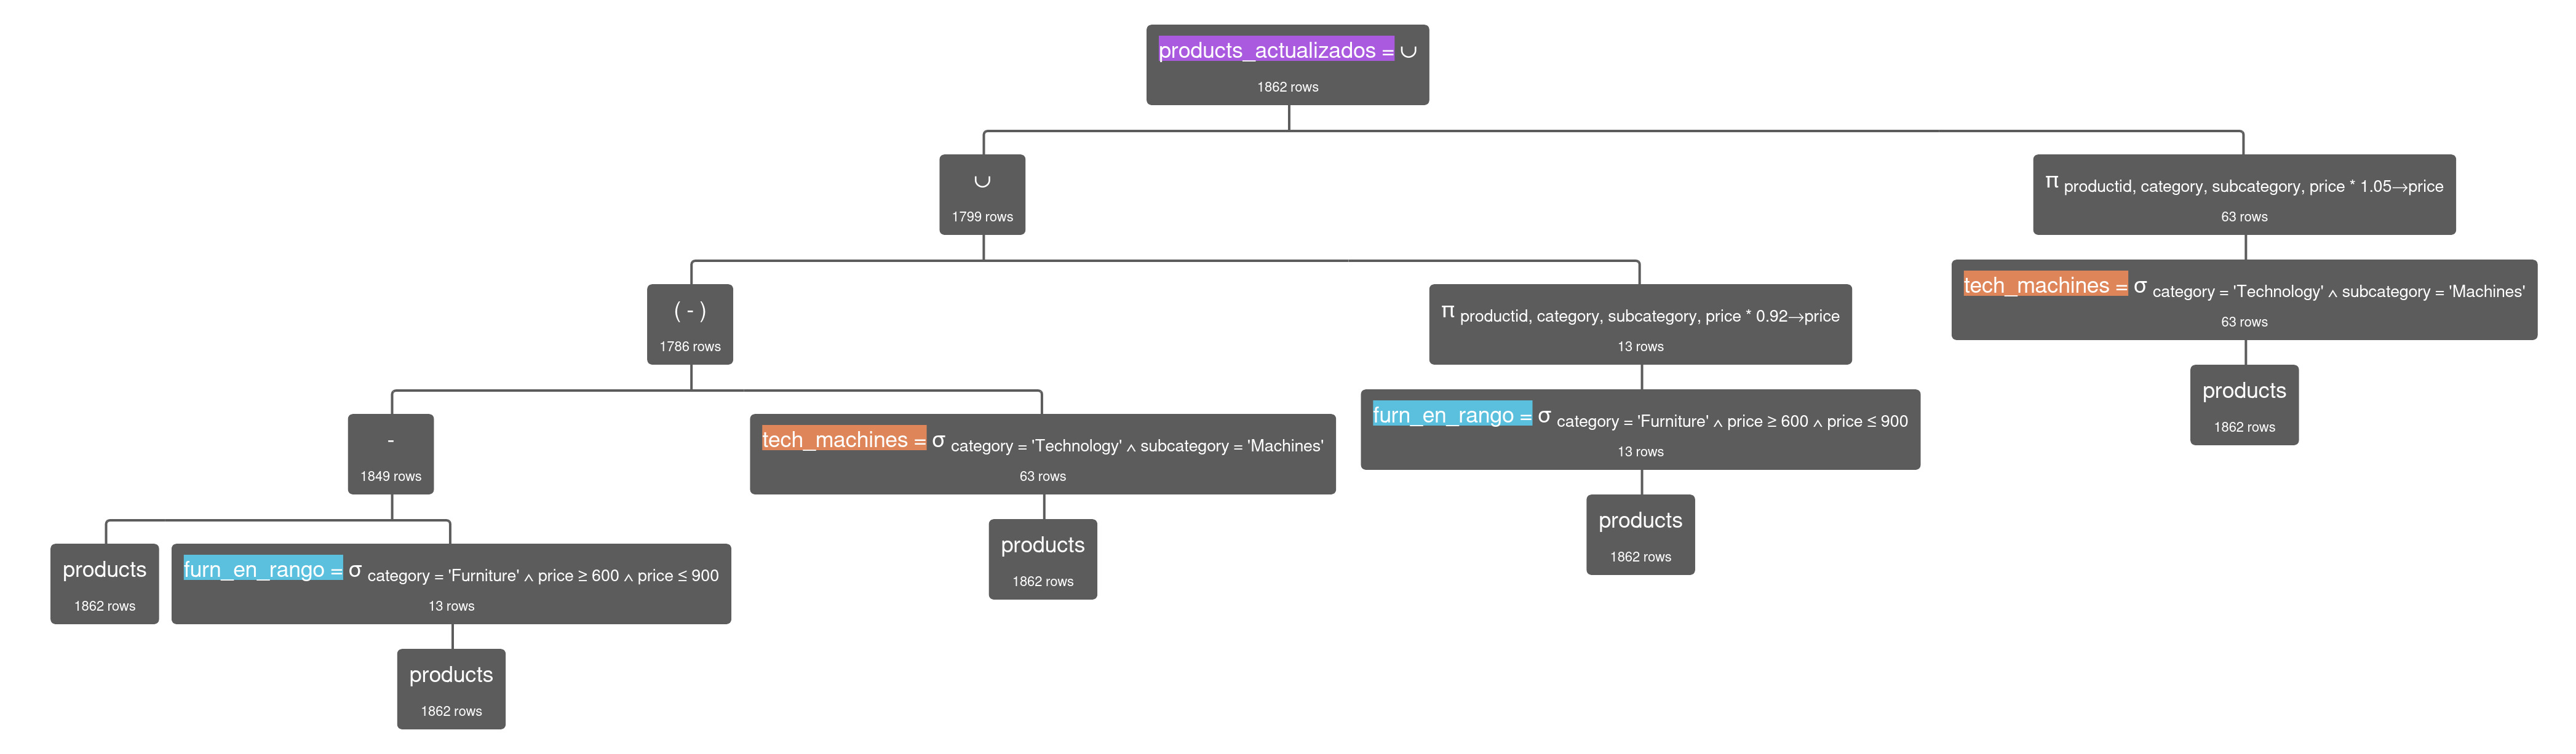
\includegraphics[width=\textwidth, height=0.38\textheight, keepaspectratio]{figuras/3e_arbol.png}

\vspace{0.35cm}
{\small Árbol de consulta de la actualización}

\vspace{0.45cm}
\begin{tabular}{@{}c@{\hspace{0.5cm}}c@{}}
\begin{minipage}[t]{0.38\textwidth}
  \centering
  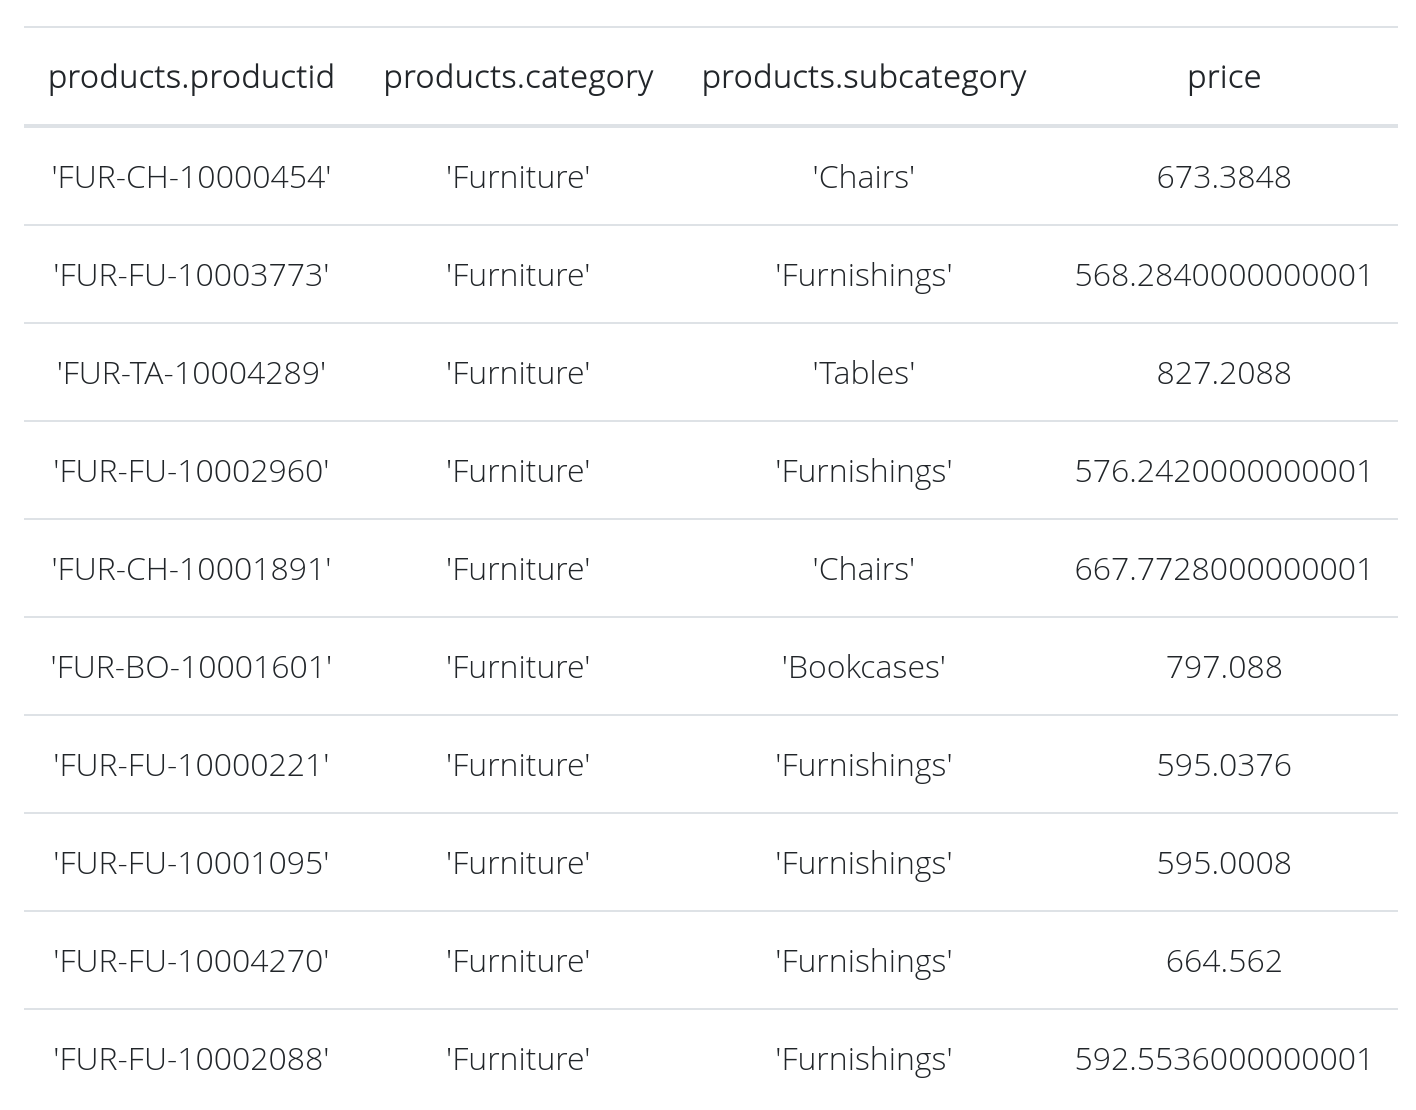
\includegraphics[width=\linewidth]{figuras/3e_tuplas_furn.png}\\[0.15cm]
  {\small Furniture actualizado}
\end{minipage} &
\begin{minipage}[t]{0.38\textwidth}
  \centering
  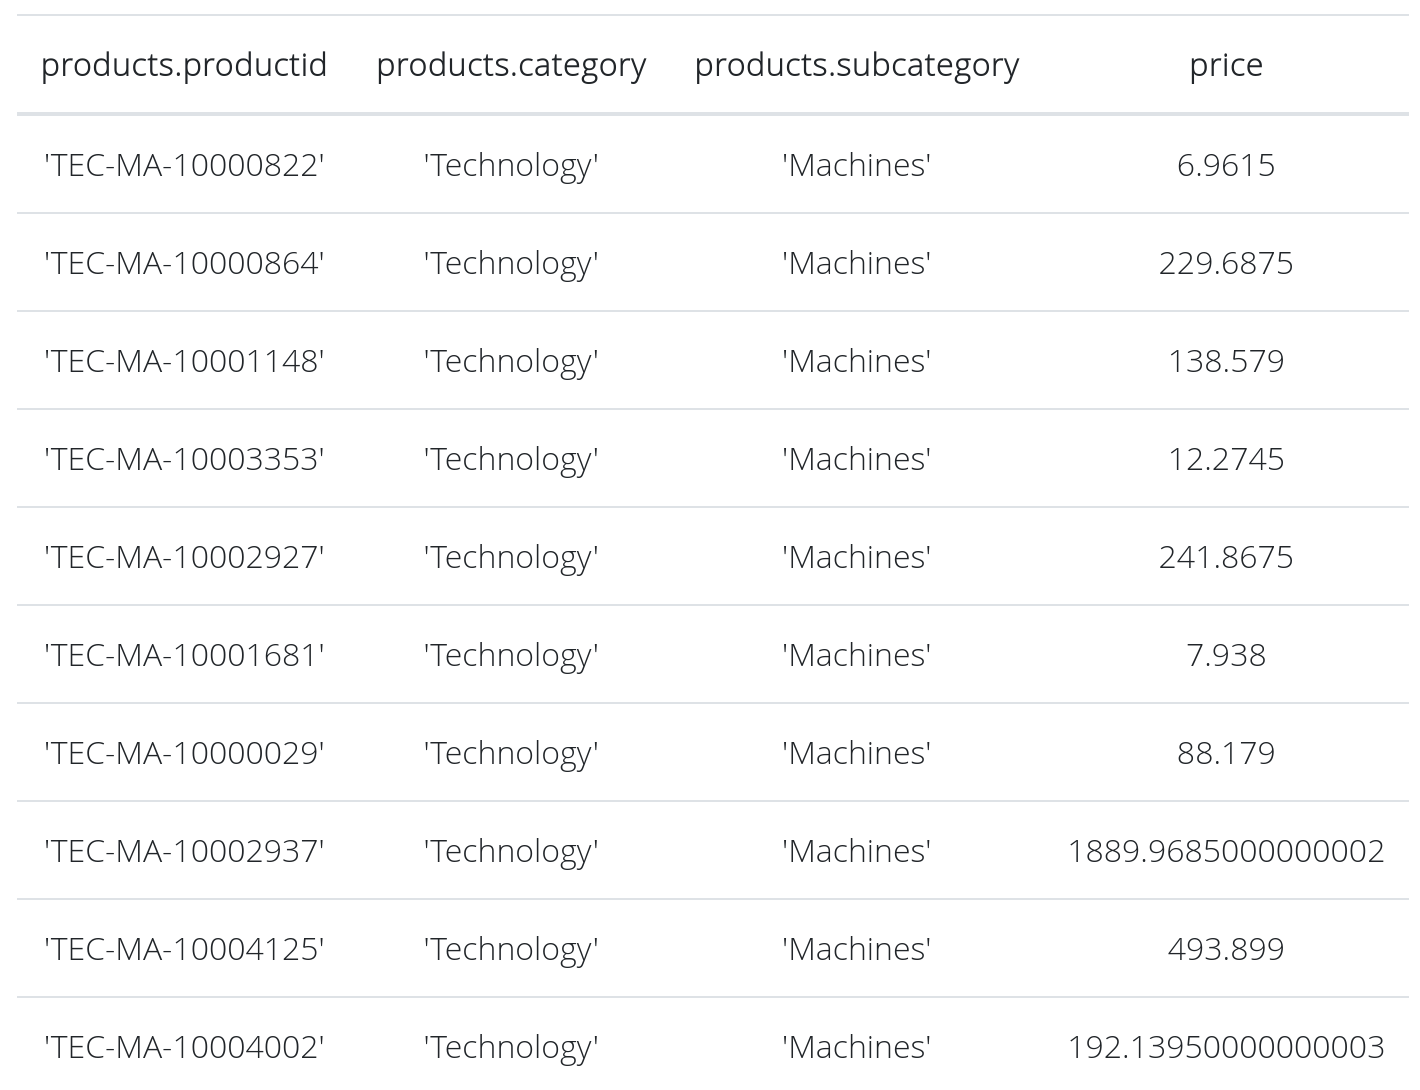
\includegraphics[width=\linewidth]{figuras/3e_tuplas_tech_machines.png}\\[0.15cm]
  {\small Technology/Machines actualizado}
\end{minipage}
\end{tabular}

\vspace{0.35cm}
{\small Las tuplas mostradas corresponden a los productos ya actualizados;
se presentan por separado porque en la tabla general de \texttt{products}
los 13 registros de \texttt{Furniture} y los 63 de
\texttt{Technology/Machines} son escasos entre 1862 renglones.}
\clearpage
\restoregeometry
\pdfpagewidth=\paperwidth
\pdfpageheight=\paperheight
